\chapter{Analysis}\label{analysis}
\lhead[\fancyplain{}{\bfseries\thepage}]{\fancyplain{}{\bfseries\rightmark}}

In this Chapter we explain the starting implementation and analysis of the model following biological considerations.

\section{Implementation}

The theoretical model was analysed making simulations using Python.
The first thing was to create a class \emph{Random Network} in order to have a random boolean graph as an object, with its own nodes and links, represented by a boolean adjacency matrix.

\begin{verbatim}
class Random_Network:
    def __init__(self, N, K):
        self.n = N
        self.k = K
        self.nodes = np.zeros((self.n,1))
        self.activity = np.sum(self.nodes)
        self.adj_matrix = np.zeros((self.n,self.n))
        if self.k == 1:
            while True:
                self.adj_matrix = np.identity(self.n)
                np.random.shuffle(self.adj_matrix)
                self.adj_matrix[np.random.randint(self.n)][np.random.randint(self.n)] = 1
                if np.trace(self.adj_matrix) == 0:
                    break
        else:
            for i in range(self.n):
                for j in range(self.k):
                    numbers = list(range(0,i)) + list(range(i+1,self.n))
                    r = random.choice(numbers)
                    self.adj_matrix[i][r] = 1
\end{verbatim}

Every random network is built in order to avoid self loops, and this mean to create a random boolean adjacency matrix with null trace.

The first thing to evalute, was to choose the mean number of incoming links for each RBN. In Figure\ref{fig:K} we can see that the mean discrete evolution of $100$ different realizations of RBNs, with increasing size.
\begin{figure}[h]
\centering
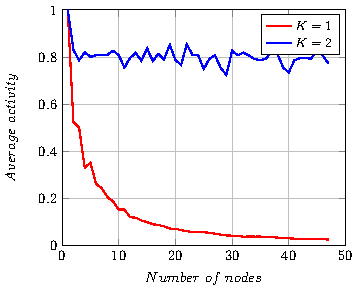
\includegraphics[scale=1.5]{images/K.pdf}
\caption{\emph{Plot of the mean activity of the nodes with network of increasing size.
In the case of $K=1$ (i.e. the mean number of incoming link for each network is one), the mean activity decreases exponentially with the size of the network; in the case of $K=2$ instead, the mean activity of the nodes remains stable with the network size.}}
\label{fig:K}
\end{figure}
In the case of $K=1$, i.e. the mean number of incoming links for each network is one, the mean activity decrease exponentially with the size of the network; in the case of $K=2$ instead, the mean activity of the nodes remains stable with the network size.

\section{Noise}
The second thing to evaluate is the effect of the noise on the evolution of the network and the difference between noise and parametric noise, where parametric noise refers to the noise which infer in the links and not on the nodes.
\begin{figure}[h]
\centering
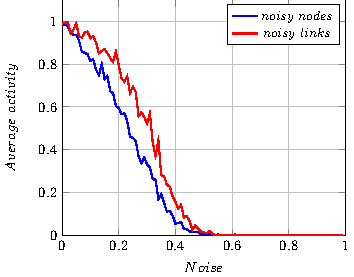
\includegraphics[scale=1.5]{images/noise.pdf}
\caption{\emph{Plot of the noise.}}
\label{fig:noise}
\end{figure}
